\documentclass[11pt,a4paper]{article}

% ---------- Packages ----------
\usepackage[utf8]{inputenc}
\usepackage[T1]{fontenc}
\usepackage[margin=2.3cm]{geometry}
\usepackage{tikz}
\usetikzlibrary{arrows.meta,positioning,fit,backgrounds,shapes.multipart,calc}
\usepackage{xcolor}
\usepackage{booktabs}
\usepackage{array}
\usepackage{longtable}
\usepackage{enumitem}
\usepackage{titlesec}
\usepackage{fancyhdr}
\usepackage{tcolorbox}
\tcbuselibrary{skins,breakable}
\usepackage{hyperref}
\usepackage{parskip}
\usepackage{ragged2e}
\usepackage{footmisc}

% ---------- Colors ----------
\definecolor{navy}{HTML}{1B2A4A}
\definecolor{teal2}{HTML}{157A6E}
\definecolor{amber}{HTML}{C97A1A}
\definecolor{crimson}{HTML}{A32638}
\definecolor{lightbg}{HTML}{F4F6F8}
\definecolor{midgray}{HTML}{5B6570}
\definecolor{greenok}{HTML}{2E7D4F}

% ---------- Section styling ----------
\titleformat{\section}{\large\bfseries\color{navy}}{\thesection}{0.5em}{}
\titleformat{\subsection}{\normalsize\bfseries\color{teal2}}{\thesubsection}{0.5em}{}
\titleformat{\subsubsection}{\normalsize\bfseries\color{midgray}}{\thesubsubsection}{0.5em}{}
\titlespacing*{\section}{0pt}{1.4em}{0.6em}
\titlespacing*{\subsection}{0pt}{1.1em}{0.4em}

% ---------- Header/Footer ----------
\pagestyle{fancy}
\fancyhf{}
\renewcommand{\headrulewidth}{0.4pt}
\renewcommand{\footrulewidth}{0.2pt}
\fancyhead[L]{\small\color{midgray} EyesOnGuj -- High-Level Design}
\fancyhead[R]{\small\color{midgray} \leftmark}
\fancyfoot[C]{\small\color{midgray} \thepage}

\hypersetup{
  colorlinks=true,
  linkcolor=teal2,
  urlcolor=teal2,
  citecolor=teal2,
  pdftitle={EyesOnGuj -- High-Level Design},
  pdfauthor={EyesOnGuj Engineering}
}

\setlist[itemize]{leftmargin=1.4em, itemsep=0.15em, topsep=0.3em}
\setlist[enumerate]{leftmargin=1.6em, itemsep=0.15em, topsep=0.3em}

% ---------- Status box helpers (implemented / partial / planned) ----------
\newtcolorbox{statusbox}[2][]{
  colback=#2!6, colframe=#2!70!black, boxrule=0.6pt, arc=1.5pt,
  left=6pt, right=6pt, top=4pt, bottom=4pt, #1
}

\newcommand{\statuschip}[2]{%
  \tikz[baseline=-0.5ex]\node[fill=#1!15, draw=#1!60!black, rounded corners=2pt,
    inner sep=3pt, font=\scriptsize\bfseries, text=#1!60!black]{#2};%
}

\newcommand{\implemented}{\statuschip{greenok}{IMPLEMENTED}}
\newcommand{\partialstat}{\statuschip{amber}{PARTIAL}}
\newcommand{\planned}{\statuschip{midgray}{PLANNED}}

% table row color helper
\newcolumntype{L}[1]{>{\RaggedRight\hspace{0pt}}p{#1}}

\begin{document}

% ======================================================================
% TITLE PAGE
% ======================================================================
\begin{titlepage}
\begin{tikzpicture}[remember picture, overlay]
  \fill[navy] (current page.north west) rectangle ([yshift=-6.2cm]current page.north east);
  \fill[teal2] (current page.north west) rectangle ([yshift=-6.0cm]current page.north east);
  \fill[navy] (current page.north west) rectangle ([yshift=-5.85cm]current page.north east);
  \node[anchor=north, text width=15cm, align=center] at ([yshift=-1.9cm]current page.north) {\color{white}\Huge\bfseries EyesOnGuj};
  \node[anchor=north, text width=13cm, align=center] at ([yshift=-3.4cm]current page.north) {\color{white}\large A Unified, Interoperable CCTV Integration and Video Analytics Platform};
\end{tikzpicture}

\vspace*{6.6cm}

\begin{center}
{\LARGE\bfseries\color{navy} High-Level Design Document}\\[0.4cm]
{\large\color{midgray} Technical Architecture, Data Model, Analytics Pipeline, Security and Scale Plan}
\end{center}

\vspace{1.8cm}

\begin{center}
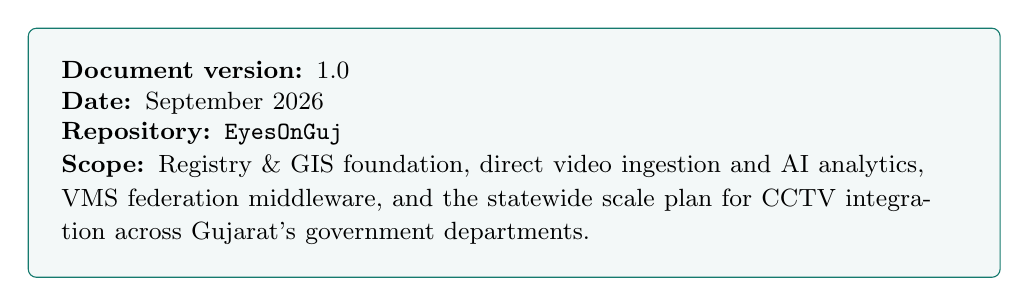
\begin{tikzpicture}
\node[draw=teal2, rounded corners=3pt, fill=teal2!5, inner sep=12pt, text width=11.5cm, align=left]{
\small
\textbf{Document version:} 1.0 \\
\textbf{Date:} September 2026 \\
\textbf{Repository:} \texttt{EyesOnGuj} \\
\textbf{Scope:} Registry \& GIS foundation, direct video ingestion and AI analytics,
VMS federation middleware, and the statewide scale plan for CCTV integration
across Gujarat's government departments.
};
\end{tikzpicture}
\end{center}

\vfill

\begin{center}
\small\color{midgray}
This document describes the system as implemented in the accompanying codebase.
Section~\ref{sec:status} states plainly which capabilities are live today,
which are partially built, and which are documented as near-term roadmap --
consistent with how the rest of this project's engineering documentation
already treats unfinished work.
\end{center}
\vspace{0.6cm}
\end{titlepage}

% ======================================================================
\tableofcontents
\thispagestyle{empty}
\newpage
\setcounter{page}{1}

% ======================================================================
\section{Purpose and Scope}

This document is the technical architecture reference for EyesOnGuj, a platform
for integrating heterogeneous, departmentally-owned CCTV infrastructure across
Gujarat into one operational picture: a shared camera registry, unified live
viewing, AI-driven vehicle and person analytics, and cross-VMS correlation
against watchlist databases, without requiring any department to replace
infrastructure it already runs and trusts.

It is written for anyone evaluating, extending, or operating the system:
what exists, why it is built the way it is, where the architectural seams are,
and what is intentionally deferred rather than silently missing. Section
\ref{sec:status} is the single most load-bearing part of this document for
that last point, and is worth reading before the rest.

The design responds to four structural facts about the problem: twenty-six
departments run independent camera estates on different vendors, VMS
platforms, storage backends and retention policies; camera sites are spread
across the state, in some cases roughly a thousand kilometres apart; any
useful analytics layer has to work uniformly across all of that
heterogeneity; and the platform has to grow from a pilot of a few dozen
cameras today toward a statewide estate on the order of eighty thousand,
without a redesign along the way.

% ======================================================================
\section{Architecture Overview}
\label{sec:arch-overview}

\subsection{Why a hybrid model}

EyesOnGuj does not commit to a single reference architecture. It combines
three of them, because the three solve three different, genuinely distinct
problems that a real statewide rollout will always have simultaneously:

\begin{itemize}
\item \textbf{Registry \& GIS foundation.} Every camera, regardless of how
  it is eventually connected, needs one authoritative record: where it is,
  who owns it, what state it's in. This has to exist independently of
  any streaming or federation decision, and every other model builds on it.
\item \textbf{Direct, middleware-free ingestion.} Where a camera or NVR is
  directly reachable over RTSP, the platform should connect straight to it.
  Adding a transcoding proxy or broker in front of a feed that doesn't need
  one is unnecessary latency, unnecessary bandwidth, and one more system
  that can fail.
\item \textbf{Federation for vendor-locked and remote VMS estates.} A
  department running a closed VMS (a Milestone, HikCentral or Dahua-class
  platform) is not going to expose raw RTSP to an outside system, and
  shouldn't have to. That estate needs an adapter that speaks the VMS's own
  protocol, or the open ONVIF standard, or a generic REST API, and reports
  into the same correlation layer as everything else.
\end{itemize}

These aren't three competing proposals picked to hedge a scoring rubric;
they are three answers to three different onboarding realities that all
show up in the same statewide estate at once. A pilot deployment can lean
almost entirely on direct RTSP because the demo cameras are reachable
directly; a real statewide rollout will need the federation layer for the
departments that don't expose raw streams. Building both from day one means
the architecture doesn't need to change shape when that mix shifts.

\subsection{System architecture}

Figure~\ref{fig:master-arch} shows the system end to end: four classes of
camera source, two onboarding paths into the platform, one shared
application core, one shared data layer, and one set of operator-facing
dashboards drawing on all of it.

\begin{figure}[h]
\centering
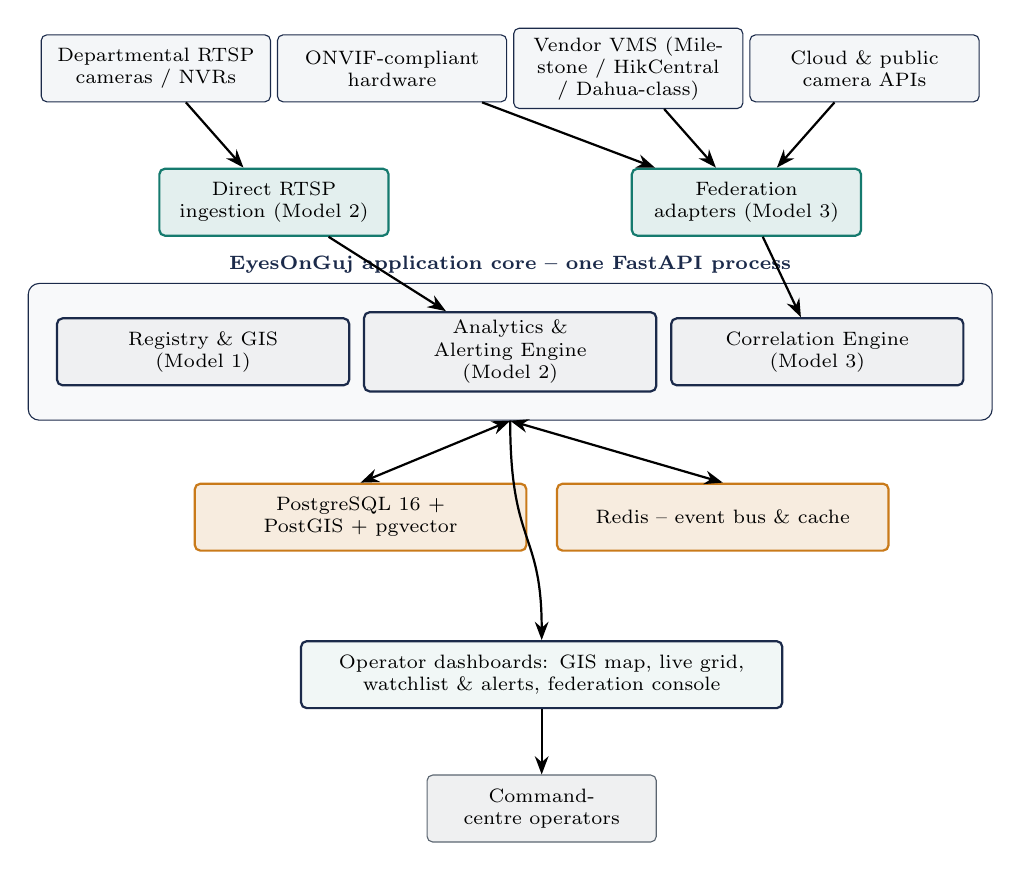
\begin{tikzpicture}[
  font=\scriptsize,
  box/.style={draw, rounded corners=2pt, minimum height=0.85cm, text width=2.7cm, align=center, inner sep=3pt},
  src/.style={box, fill=lightbg, draw=navy, thin},
  ingest/.style={box, fill=teal2!12, draw=teal2},
  coreb/.style={draw, rounded corners=2pt, fill=navy!7, draw=navy, minimum height=0.85cm, text width=3.5cm, align=center, inner sep=3pt},
  data/.style={box, fill=amber!14, draw=amber, text width=4cm},
  dashb/.style={box, fill=teal2!6, draw=navy, text width=5.9cm},
  >=Stealth, thick
]

% ---- Row 0: sources ----
\node[src] (s1) at (0,7.2)   {Departmental RTSP cameras / NVRs};
\node[src] (s2) at (3.0,7.2) {ONVIF-compliant hardware};
\node[src] (s3) at (6.0,7.2) {Vendor VMS (Milestone / HikCentral / Dahua-class)};
\node[src] (s4) at (9.0,7.2) {Cloud \& public camera APIs};

% ---- Row 1: ingestion paths ----
\node[ingest] (m2) at (1.5,5.5) {Direct RTSP ingestion (Model 2)};
\node[ingest] (m3) at (7.5,5.5) {Federation adapters (Model 3)};

\draw[->] (s1) -- (m2);
\draw[->] (s2) -- (m3);
\draw[->] (s3) -- (m3);
\draw[->] (s4) -- (m3);

% ---- Row 2: application core ----
\node[coreb] (c1) at (0.6,3.6)  {Registry \& GIS\\ (Model 1)};
\node[coreb] (c2) at (4.5,3.6)  {Analytics \& Alerting Engine\\ (Model 2)};
\node[coreb] (c3) at (8.4,3.6)  {Correlation Engine\\ (Model 3)};

\begin{scope}[on background layer]
\node[draw=navy, rounded corners=4pt, fill=navy!3, fit=(c1)(c2)(c3), inner sep=10pt, label={[navy,font=\scriptsize\bfseries]above:EyesOnGuj application core -- one FastAPI process}] (coreband) {};
\end{scope}

\draw[->] (m2) -- (c2);
\draw[->] (m3) -- (c3);

% ---- Row 3: data layer ----
\node[data] (db) at (2.6,1.5) {PostgreSQL 16 + PostGIS + pgvector};
\node[data] (redis) at (7.2,1.5) {Redis -- event bus \& cache};

\draw[<->] (coreband.south) -- (db.north);
\draw[<->] (coreband.south) -- (redis.north);

% ---- Row 4: dashboards ----
\node[dashb] (dash1) at (4.9,-0.5) {Operator dashboards: GIS map, live grid, watchlist \& alerts, federation console};

\draw[->] (coreband.south) .. controls +(0,-1.6) and +(0,1.4) .. (dash1.north);

% ---- Row 5: operators ----
\node[src, fill=midgray!10, draw=midgray] (ops) at (4.9,-2.2) {Command-centre operators};
\draw[->] (dash1) -- (ops);

\end{tikzpicture}

\caption{System architecture: sources, ingestion paths, application core,
data layer, and operator dashboards.}
\label{fig:master-arch}
\end{figure}

The load-bearing decision in this diagram is that both ingestion paths feed
the \emph{same} application core, the same PostgreSQL schema, and the same
correlation logic. A vehicle detection from a directly-ingested RTSP feed
and a detection event relayed through a federated VMS adapter land in the
same \texttt{detections} table, get correlated against the same watchlist,
and can be joined into the same cross-camera route. There is no "federated
data" silo sitting apart from "direct" data; a camera is a camera and a
sighting is a sighting, regardless of which door it came in through.

\subsection{Deployment shell}

All three models run inside one FastAPI application process rather than as
three separate services. This is a deliberate simplification, not a
shortcut: it means one login session, one role-based access control layer,
one template engine, and one deployment unit, instead of three services
that all have to independently agree on how authentication works. The
trade-off, and it is a real one, is that scaling the application means
scaling one process rather than scaling each concern independently; Section
\ref{sec:scale} addresses how that trade-off is managed as camera count
grows.

% ======================================================================
\section{Camera Onboarding and Integration Strategy}
\label{sec:integration}

Heterogeneity is the first-order problem this platform exists to solve, and
it is treated as a routing decision rather than a special case handled ad
hoc per vendor. Table~\ref{tab:onboarding-paths} summarises how a camera,
NVR, or VMS estate enters the platform depending on what it actually
exposes.

\begin{table}[h]
\centering
\small
\begin{tabular}{L{3.0cm}L{4.0cm}L{4.2cm}L{2.6cm}}
\toprule
\textbf{Source type} & \textbf{Onboarding path} & \textbf{Mechanism} & \textbf{Code path} \\
\midrule
Directly-reachable RTSP camera / NVR & Direct ingestion & Supervisor spins up one stream worker per camera, forced over TCP & Model 2 \\
ONVIF-compliant camera or NVR & Federation, config-driven & SOAP over ONVIF Media/Device WSDL; one onboarded system can represent a multi-channel NVR & Model 3 \\
Closed vendor VMS (Milestone / HikCentral / Dahua-class) & Federation, adapter self-registration & Vendor-specific adapter translating the VMS's own event shape into a canonical event schema & Model 3 \\
Cloud or public REST camera API (e.g.\ Windy-class webcam directories) & Federation, config-driven & Generic REST + API-key adapter with dotted-path field mapping, no new code per vendor & Model 3 \\
Bulk metadata (CSV) or manual entry, no live feed & Registry only & Camera exists as a registry row; connects to streaming or federation later if a feed becomes available & Model 1 \\
\bottomrule
\end{tabular}
\caption{Onboarding path by source type.}
\label{tab:onboarding-paths}
\end{table}

\subsection{The adapter pattern}

Every VMS integration in Model 3 implements one interface: \texttt{connect}, \texttt{get\_cameras},
and \texttt{start\_event\_stream}. Table~\ref{tab:vendor-shapes}
shows why this matters in practice, not just in principle: three vendor
payload shapes for the same underlying concept, a license-plate detection
event, disagree on nearly every field name and even the timestamp encoding.

\begin{table}[h]
\centering
\small
\begin{tabular}{lccc}
\toprule
\textbf{Field} & \textbf{Milestone-class} & \textbf{HikCentral-class} & \textbf{Dahua-class} \\
\midrule
Plate & \texttt{licensePlate} & \texttt{plateText} & \texttt{plate} \\
Confidence & \texttt{score} & \texttt{detectionConfidence} & \texttt{conf} \\
Timestamp & ISO-8601 & ISO-8601 & Unix integer \\
Camera ID & \texttt{deviceId} & \texttt{cameraIndex} & \texttt{channel} \\
Push model & XML/SDK event push & REST subscription & WebSocket push \\
\bottomrule
\end{tabular}
\caption{Representative field-naming divergence across three vendor VMS payload shapes -- the concrete shape of the interoperability problem this platform solves.}
\label{tab:vendor-shapes}
\end{table}

Each adapter normalises its vendor's shape into one canonical event schema
before anything downstream ever sees it. Onboarding a new \emph{vendor that
already speaks a supported protocol} -- any ONVIF-compliant device, or any
REST service returning a JSON array of camera-like objects -- needs zero
new code: the adapter registry exposes a configuration form (host,
credentials, field paths) and a live \emph{Test Connection} check before
anything is persisted. Onboarding a new \emph{protocol} still needs one new
adapter class written once, which is an honest property of protocols being
genuinely different things, not a gap in the framework.

\subsection{One camera table, three contributors}

A single \texttt{cameras} table is the shared source of truth across all
three models, carrying three distinct groups of columns that different
parts of the system populate:

\begin{itemize}
\item \textbf{Registry fields} -- department, district, location, ownership,
  storage type, retention period. Owned by Model 1, editable by a
  department administrator.
\item \textbf{Grid-sync fields} -- codec, resolution, bitrate, stream URLs.
  Populated automatically by Model 2's catalogue poller against the
  government camera grid's own inventory API; Model 1 reads these but never
  writes them.
\item \textbf{VMS linkage} -- a foreign key into \texttt{vms\_systems}, the
  join point Model 3 uses to tie a registry row to the specific federated
  VMS connection that reported it. \texttt{NULL} means the camera came from
  the main grid or was onboarded manually; a non-null value traces it back
  to exactly which departmental VMS reported it.
\end{itemize}

A camera onboarded through any of these three paths shows up identically on
the GIS map, in the live grid, and in gap-analysis reporting -- there is no
second-class camera depending on which door it came in through.

% ======================================================================
\section{Registry and GIS Foundation}
\label{sec:model1}

The registry answers the question no department currently has a
consolidated answer to: what cameras actually exist, where, whose are they,
and can that record be trusted. It is deliberately registry-only -- it does
not stream or store video -- so that it can exist as a stable foundation
underneath whichever streaming or federation approach a given camera
ultimately uses.

\subsection{Data model}

\begin{itemize}
\item \texttt{departments} -- department name and category, seed data.
\item \texttt{districts} -- Gujarat's 33 administrative districts with real
  polygon boundaries, sourced from a public administrative-boundary
  dataset and matched by official Local Government Directory codes rather
  than by name, so the mapping is unambiguous.
\item \texttt{cameras} -- the core registry payload (Section~\ref{sec:integration}).
\item \texttt{status\_history} -- one row per tracked field change, written
  by a database trigger rather than application code, so audit logging
  cannot be silently skipped by a code path that forgets to call it.
\end{itemize}

District boundaries are simplified with a topology-aware algorithm run once
across the whole set of 33 districts rather than polygon by polygon, so
that neighbouring districts keep the exact same shared edge instead of two
independently-rounded approximations of it. That matters directly for the
gap-analysis computation below, which depends on those boundaries being
geometrically consistent, not just visually acceptable on a map.

\subsection{Coverage gap analysis}

This is the one place the registry performs real spatial computation rather
than serving pins on a map:

\begin{enumerate}
\item Every active, located camera gets a circular buffer computed as a true
  geodesic distance (accounting for the earth's curvature), not a flat-plane
  approximation.
\item All of one district's buffers are merged into a single coverage shape.
\item That coverage shape is subtracted from the district's own boundary --
  what remains is the actual uncovered area, as a polygon, not just a
  percentage.
\item The uncovered area is measured against the district's total area to
  produce a coverage percentage, sorted worst-covered first.
\end{enumerate}

The whole computation runs as a single spatial SQL query across all 33
districts at once, letting the database's own spatial engine parallelise
the work, rather than looping over cameras in application code. This is
the difference that matters once camera counts climb into the thousands:
per-row overhead in application code does not scale the way a set-based
database query does.

\subsection{Role-based UI and audit trail}

Camera markers on the map use custom, status- and department-specific
iconography rather than tinted default pins, deliberately, because the map
is the page an operator watches continuously during a shift; distinguishing
"is anything offline right now" at a glance matters more here than almost
anywhere else in the product. Bulk CSV onboarding, manual entry, and
role-scoped editing all write through the same audit trigger described
above, and a department administrator can only create or edit cameras
within their own department -- enforced at the API layer, not just hidden
in the UI (Section~\ref{sec:security}).

% ======================================================================
\section{Unified Viewing and Direct Video Ingestion}
\label{sec:model2}

Model 2 answers the operational question: how does a command-centre
operator watch and run analytics across dozens of independent departmental
camera systems at once, without replacing any department's own VMS and
without re-recording every camera's raw video into central storage.

\subsection{Streaming architecture}

The platform connects directly to each reachable camera over RTSP,
forced over TCP for reliability, and re-serves it to operators over three
paths depending on what the browser can consume: low-latency WebRTC (WHEP)
for live preview, HLS for the multi-camera grid wall, and a server-side
MJPEG relay as a codec-agnostic fallback. No transcoding proxy or broker
sits between the camera and the first hop of this pipeline -- what the
camera outputs is what the ingestion worker reads.

\begin{statusbox}{teal2}
\textbf{Decoupled ingestion.} Stream capture and AI inference cannot share
the same event loop: decoding video over a variable-latency network would
block every other request the application serves. An ingestion supervisor
runs one capture worker per active camera, feeding a bounded in-memory
frame queue that the inference stage reads independently. If inference
falls behind, frames are dropped rather than buffered -- the pipeline
processes what is happening now, not a growing backlog of what happened a
few seconds ago.
\end{statusbox}

\subsection{Selective metadata, not bulk video}

Centralising raw video from a statewide camera estate does not scale --
storage grows linearly with camera count and retention period regardless
of whether anything interesting ever happened on a given feed. EyesOnGuj
takes the opposite approach: raw frames are evaluated in memory and
discarded immediately after inference. Only structured, high-value output
is persisted -- bounding boxes, normalised plate strings, cropped
thumbnails, track identifiers, and watchlist match records. The practical
consequence is that central storage grows with \emph{incidents}, not with
\emph{camera count} or \emph{elapsed time}, which is the only version of
this that is actually compatible with an eighty-thousand-camera target.

\subsection{Dual ingestion: live and forensic}

The same three-stage analytics pipeline (Section~\ref{sec:analytics})
processes two independent input sources:

\begin{itemize}
\item \textbf{Live feeds} -- camera workers run on demand, starting when an
  operator opens the live detection view and stopping when the last client
  disconnects, rather than running continuously in the background regardless
  of whether anyone is watching.
\item \textbf{Forensic upload} -- investigators can upload recorded footage
  (up to 2\,GB) for the same pipeline to process at adjustable playback
  speed, with pause, resume and stop controls, on an isolated worker thread
  that never competes with live ingestion for resources.
\end{itemize}

% ======================================================================
\section{VMS Federation and Middleware}
\label{sec:model3}

Where Section~\ref{sec:model2} connects directly to a reachable stream,
Model 3 is the layer that reaches departments whose cameras sit behind a
closed VMS or a remote API. Architecturally the two are peers, not a
pipeline: Model 3 does not sit in front of Model 2's traffic, and Model 2's
live pipeline has no runtime dependency on Model 3 being available.

\subsection{Event bus and correlation engine}

Every adapter, regardless of vendor, publishes a normalised event onto a
single publish/subscribe channel. One background correlation engine
subscribes to that channel and runs the same pipeline for every event
(Figure~\ref{fig:correlation-flow}):

\begin{enumerate}
\item \textbf{Deduplicate} -- the same plate from the same camera within a
  short window is collapsed to one event.
\item \textbf{Resolve the camera} -- look up the registry row for this VMS
  and this camera's external id; an event for a camera that was never
  registered is logged and dropped rather than inserted with a fabricated
  reference.
\item \textbf{Resolve or create the vehicle track} -- derived deterministically
  from the normalised plate, using the \emph{same derivation} Model 2's own
  analytics pipeline uses, so a plate resolves to the same track whether
  Model 2's direct pipeline or a federated adapter saw it first.
\item \textbf{Watchlist check}, before the sighting is written, so a match is
  known at insert time.
\item \textbf{Persist the sighting} with full raw-payload audit trail.
\item \textbf{Alert on a match}, broadcast immediately over WebSocket.
\item \textbf{Cross-system correlation} -- has this same vehicle track been
  seen through a \emph{different} VMS recently? If so, broadcast the full
  camera sequence it travelled through. This is never stored separately;
  it is always recomputed from the raw sightings, so it can never drift
  from what was actually observed.
\item \textbf{Broadcast the event} to every connected dashboard.
\end{enumerate}

\begin{figure}[h]
\centering
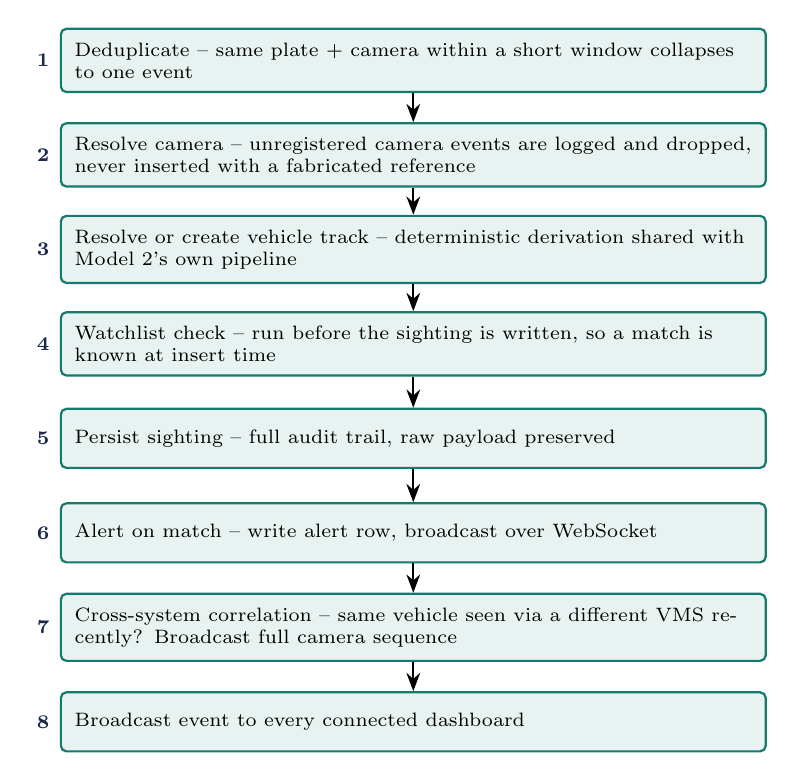
\begin{tikzpicture}[
  font=\scriptsize,
  flowstep/.style={draw, rounded corners=2pt, fill=teal2!10, draw=teal2, minimum height=0.75cm, text width=8.6cm, align=left, inner sep=5pt},
  >=Stealth, thick
]

\node[flowstep, label=left:{\scriptsize\bfseries\color{navy}1}] (nA) at (0,7.5) {Deduplicate -- same plate + camera within a short window collapses to one event};
\node[flowstep, label=left:{\scriptsize\bfseries\color{navy}2}] (nB) at (0,6.3) {Resolve camera -- unregistered camera events are logged and dropped, never inserted with a fabricated reference};
\node[flowstep, label=left:{\scriptsize\bfseries\color{navy}3}] (nC) at (0,5.1) {Resolve or create vehicle track -- deterministic derivation shared with Model 2's own pipeline};
\node[flowstep, label=left:{\scriptsize\bfseries\color{navy}4}] (nD) at (0,3.9) {Watchlist check -- run before the sighting is written, so a match is known at insert time};
\node[flowstep, label=left:{\scriptsize\bfseries\color{navy}5}] (nE) at (0,2.7) {Persist sighting -- full audit trail, raw payload preserved};
\node[flowstep, label=left:{\scriptsize\bfseries\color{navy}6}] (nF) at (0,1.5) {Alert on match -- write alert row, broadcast over WebSocket};
\node[flowstep, label=left:{\scriptsize\bfseries\color{navy}7}] (nG) at (0,0.3) {Cross-system correlation -- same vehicle seen via a different VMS recently? Broadcast full camera sequence};
\node[flowstep, label=left:{\scriptsize\bfseries\color{navy}8}] (nH) at (0,-0.9) {Broadcast event to every connected dashboard};

\draw[->] (nA) -- (nB);
\draw[->] (nB) -- (nC);
\draw[->] (nC) -- (nD);
\draw[->] (nD) -- (nE);
\draw[->] (nE) -- (nF);
\draw[->] (nF) -- (nG);
\draw[->] (nG) -- (nH);

\end{tikzpicture}

\caption{Correlation engine pipeline, run once per event by a single background task subscribed to the event bus.}
\label{fig:correlation-flow}
\end{figure}

The event bus itself degrades gracefully: if the message broker is
unreachable, publishing falls back to a bounded in-process queue with a
logged warning, so a bare local environment with no broker running still
works end to end rather than crashing on startup.

\subsection{No separate federation schema}

An earlier design gave Model 3 its own private tables. That was dropped:
a camera reported by a federated VMS and a camera in the main registry
were becoming two different rows for the same real-world object. Model 3
now writes into exactly the same \texttt{cameras}, \texttt{detections},
\texttt{vehicle\_tracks}, and \texttt{alerts} tables that Model 1 and Model
2 already own, tagged with which VMS reported them. The practical payoff:
a full multi-system route for one plate, spanning the main grid, Model 2's
own pipeline, and every federated VMS, is one query joining tables that
already exist -- not a second correlation mechanism that has to be kept in
sync with the first.

% ======================================================================
\section{AI Video Analytics Pipeline}
\label{sec:analytics}

\subsection{Vehicle detection, tracking and ANPR}

\begin{figure}[h]
\centering
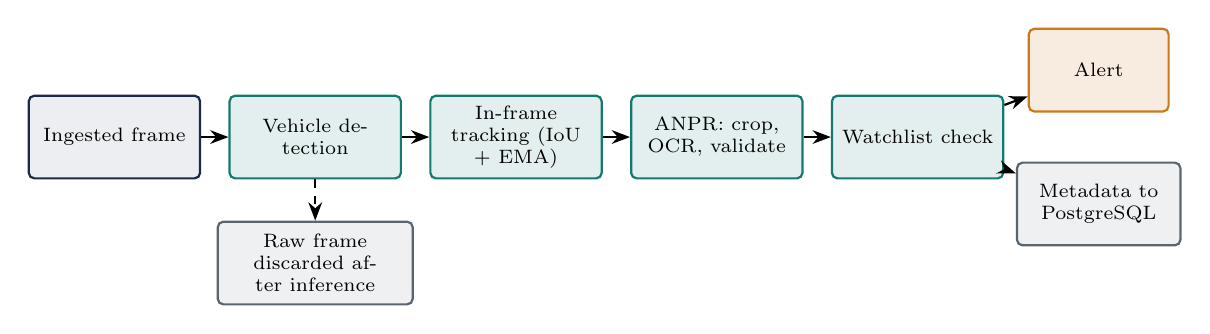
\begin{tikzpicture}[
  font=\scriptsize,
  box/.style={draw, rounded corners=2pt, minimum height=1.05cm, text width=2.0cm, align=center, inner sep=2.5pt},
  stage/.style={box, fill=teal2!12, draw=teal2},
  term/.style={box, fill=amber!14, draw=amber, text width=1.6cm},
  discard/.style={box, fill=midgray!10, draw=midgray, text width=1.9cm},
  >=Stealth, thick
]

\node[box, fill=navy!8, draw=navy] (frame) at (0,0) {Ingested frame};
\node[stage] (det) at (2.55,0) {Vehicle detection};
\node[stage] (trk) at (5.1,0) {In-frame tracking (IoU + EMA)};
\node[stage] (anpr) at (7.65,0) {ANPR: crop, OCR, validate};
\node[stage] (wl) at (10.2,0) {Watchlist check};
\node[term] (alert) at (12.5,0.85) {Alert};
\node[discard] (store) at (12.5,-0.85) {Metadata to PostgreSQL};

\draw[->] (frame) -- (det);
\draw[->] (det) -- (trk);
\draw[->] (trk) -- (anpr);
\draw[->] (anpr) -- (wl);
\draw[->] (wl) -- (alert);
\draw[->] (wl) -- (store);

\node[discard, text width=2.3cm] (raw) at (2.55,-1.6) {Raw frame discarded after inference};
\draw[->, dashed] (det) -- (raw);

\end{tikzpicture}

\caption{Three-stage vehicle analytics pipeline, run on every ingested frame.}
\label{fig:analytics-pipeline}
\end{figure}

\begin{enumerate}
\item \textbf{Vehicle detection.} Generic detectors trained on Western
  traffic distributions underperform on Indian roads, so detection uses a
  model fine-tuned on Indian traffic categories specifically: cars,
  auto-rickshaws, motorcycles and scooters, buses, trucks, mini-trucks, and
  bicycles.
\item \textbf{In-frame tracking.} Raw per-frame detections flicker and
  duplicate; a lightweight tracker assigns persistent identifiers within a
  single camera's field of view using spatial proximity and box overlap,
  with smoothing applied across frames and a minimum number of confirmed
  frames before a detection is promoted to a tracked object.
\item \textbf{ANPR.} Vehicle crops are routed to plate detection and OCR,
  and the recognised string is normalised and validated against standard
  Indian state-series and Bharat-series plate formats before being accepted.
\end{enumerate}

Cross-camera route reconstruction -- distinct from the in-frame tracking
above -- currently joins sightings primarily by normalised plate string and
timestamp, with a fallback path for appearance-based re-identification
planned for cases where OCR fails at one camera along the route. This
sequencing choice is deliberate: given a working plate pipeline, a
plate-string join already delivers genuine multi-camera route
reconstruction, and full visual re-identification becomes an enhancement
rather than a blocker for the core capability. Section~\ref{sec:status}
states this distinction plainly.

\subsection{Biometric face-matching}

A second, independent pipeline handles person-of-interest matching,
decoupled from vehicle analytics so that a facility-security or
missing-persons use case does not compete for the same code path as
traffic monitoring:

\begin{itemize}
\item \textbf{Registration.} A reference photo passes a five-gate quality
  check (face count, sharpness, pose angle within tolerance, and two
  further checks) before an embedding is generated, so a poor-quality
  reference photo is rejected at registration time rather than producing an
  unreliable watchlist entry later.
\item \textbf{Embedding.} A 512-dimensional face embedding is stored
  alongside the registry record, indexed for fast approximate nearest-
  neighbour search.
\item \textbf{Matching.} Detected faces in a video stream are embedded and
  compared against the active watchlist by cosine similarity; a match above
  the configured similarity threshold generates an alert. Non-matching
  embeddings and crops are discarded immediately -- the platform does not
  retain a biometric record of anyone who is not a match against an
  authorised watchlist.
\end{itemize}

\subsection{Evaluation discipline}

Every analytics stage is evaluated on precision, recall and F1, not a
single accuracy figure. This matters specifically because watchlist hits
are rare events against overall traffic volume: a model that predicts "no
match" on everything scores misleadingly well on raw accuracy while being
operationally useless. Detection, plate-read accuracy (character-level and
full-plate exact-match, reported separately, since a plate that is
90\% correct character-by-character is a 0\% useful match), and watchlist
alerting are each measured against a held-out, hand-labelled test set
rather than reported as a single headline number.

% ======================================================================
\section{Watchlist Correlation and Real-Time Alerting}
\label{sec:alerting}

\subsection{Data model}

\begin{table}[h]
\centering
\small
\begin{tabular}{L{3.0cm}L{9.5cm}}
\toprule
\textbf{Table} & \textbf{Role} \\
\midrule
\texttt{vehicles\_watchlist} & Target plates: category (stolen / wanted / blacklisted), reporting department, status \\
\texttt{persons\_watchlist} & Target individuals with reference embeddings and quality metrics \\
\texttt{detections} & Every instantaneous sighting, vehicle or otherwise, with camera, timestamp, and confidence \\
\texttt{vehicle\_tracks} & Synthesised cross-camera journeys, joining detections by resolved identity \\
\texttt{alerts} / \texttt{person\_alerts} & Auditable incidents: watchlist id, severity, acknowledging operator and timestamp \\
\bottomrule
\end{tabular}
\caption{Core watchlist and alerting tables, shared across all three models.}
\end{table}

An alert is not a boolean flag on a detection row; it is its own
auditable entity with a required acknowledging operator, so an alert
cannot be silently dismissed without a record of who addressed it.

\subsection{Severity and notification workflow}

\begin{table}[h]
\centering
\small
\begin{tabular}{lll}
\toprule
\textbf{Watchlist category} & \textbf{Severity} & \textbf{Operator-facing behaviour} \\
\midrule
Stolen & Critical & High-visibility alert, prioritised in the incident queue \\
Wanted & High & Flagged indicator on the live feed, prioritised queue entry \\
Blacklisted & Medium & Logged and surfaced, lower visual priority \\
\bottomrule
\end{tabular}
\caption{Severity derivation by watchlist category.}
\end{table}

On a match, the alert is written and broadcast over WebSocket to every
connected dashboard in well under a second, and stays in an
\emph{unacknowledged} state until an operator acts on it. Acknowledgement
is idempotent by design, so multiple control-room desks viewing the same
incident feed cannot race each other into an inconsistent state.

\subsection{Why plate normalisation matters here specifically}

Plate strings are normalised (whitespace, punctuation and case stripped)
before every watchlist comparison, because the comparison is only as
reliable as the string on both sides of it. This is a small implementation
detail with an outsized effect on the number that actually matters for
this platform: alerting precision and recall (Section~\ref{sec:analytics}).

% ======================================================================
\section{Security, Privacy and Auditability}
\label{sec:security}

\subsection{Authentication and session handling}

Sessions are JSON Web Tokens carried in an \texttt{httpOnly} cookie rather
than browser storage, which closes off an entire class of script-based
token theft; a bearer-token header is also accepted for direct API access.
Passwords are hashed with bcrypt and never stored or logged in reversible
form. Tokens are short-lived (an eight-hour session, matched to an
operator's shift length rather than a long-lived API credential), and the
signing key has a fail-fast check: the application refuses to start in a
production configuration if it detects the checked-in development default
key is still active, rather than silently signing real sessions with a key
that is public in the repository.

\subsection{Role-based access control}

Three roles, enforced at the API dependency layer rather than hidden in
the UI: a department administrator with full camera and watchlist CRUD
scoped to their own department, an operator with read access plus
day-to-day monitoring and alert handling, and a read-only viewer explicitly
excluded from audit-log access. Department scoping is layered on top of
role checking, not a replacement for it -- an administrator cannot create,
edit, or view detail for a camera outside their own department, and bulk
CSV import enforces the same rule per row rather than per file.

\subsection{Login rate limiting}

Failed login attempts are tracked per client-IP-and-username pair rather
than per username alone, so an attacker cannot remotely lock a real user
out of their own account by deliberately failing that user's login from an
arbitrary address. Five failures in five minutes locks that pair out for
fifteen minutes; a successful login clears the count. This is intentionally
simple, in-process state, appropriate for a single-instance deployment --
Section~\ref{sec:scale} notes explicitly where this needs to move to a
shared backend once the application scales horizontally.

\subsection{Audit trail}

Every tracked change to a camera record is written by a database trigger,
not by application code calling a logging function -- which means there is
no code path that can mutate a camera and simply forget to log it. The
same acknowledgement-based audit pattern extends to alert handling: every
alert records who acknowledged it and when.

\subsection{Sensitive media access}

Detection crop images and face-match crops are frames pulled from live
surveillance and are treated accordingly: they are not served through a
generic static-file mount, which has no way to require a login before
handing back a file. A dedicated route checks the requester is
authenticated and that the requested path cannot escape its own storage
directory before ever touching the filesystem -- the one directory that
actually holds sensitive imagery gets the one route that actually checks
who is asking.

\subsection{Transport security}

TLS termination sits in front of the application at the reverse-proxy
layer; the application itself speaks plain HTTP only on the private network
behind it. The session cookie's \texttt{secure} flag tracks the same
production/debug switch the rest of the configuration uses, so it cannot
drift out of sync with whether TLS is actually in front of it.

\subsection{What is documented here but not yet built}

Stated plainly, in the same spirit the rest of this project's engineering
documentation already uses for unfinished work, rather than left implicit:

\begin{itemize}
\item \textbf{At-rest encryption} for watchlist and detection tables
  specifically -- flagged as a pre-production requirement, not implemented
  in the current build.
\item \textbf{Encryption for stored VMS credentials.} Config-driven VMS
  onboarding can hold real credentials (an API key, a device username and
  password); today that configuration is stored as plain structured data,
  readable by anything with database access. The intended fix is
  application-layer encryption with the key held outside the database, or
  moving the secret itself into a proper secrets manager and storing only a
  reference here -- before this holds a real department's credentials
  rather than a demo key.
\item \textbf{Network segmentation} between the VMS-ingestion network and
  the public dashboard network -- described in the deployment architecture
  (Section~\ref{sec:scale}), not yet physically separated in the current
  single-host deployment.
\item \textbf{Edge-level API gateway / rate limiting}, distinct from the
  login-specific limiter above -- the statewide-scale answer to abusive
  traffic generally, not needed at pilot scale.
\end{itemize}

% ======================================================================
\section{Deployment Architecture and Statewide Scale Plan}
\label{sec:scale}

\subsection{Current deployment}

\begin{figure}[h]
\centering
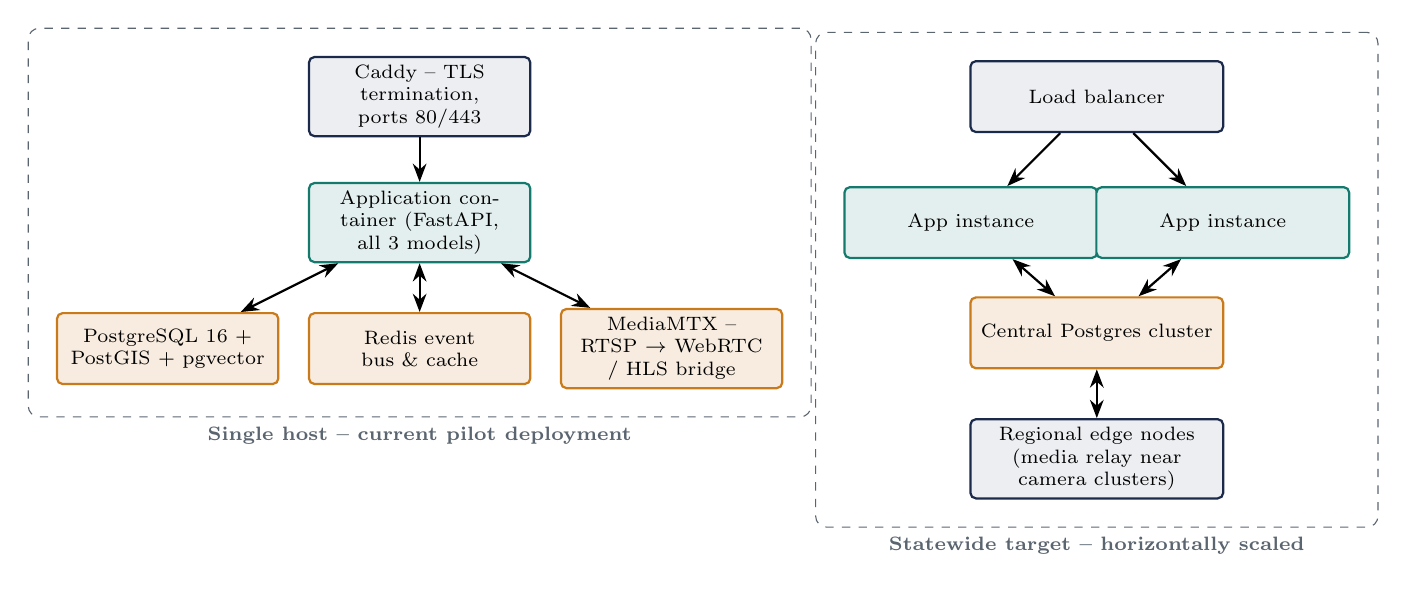
\begin{tikzpicture}[
  font=\scriptsize,
  box/.style={draw, rounded corners=2pt, minimum height=0.9cm, text width=2.6cm, align=center, inner sep=3pt},
  svc/.style={box, fill=teal2!12, draw=teal2},
  edgeb/.style={box, fill=navy!8, draw=navy},
  datab/.style={box, fill=amber!14, draw=amber},
  >=Stealth, thick
]

\node[edgeb] (caddy) at (0,3.2) {Caddy -- TLS termination, ports 80/443};
\node[svc] (app) at (0,1.6) {Application container (FastAPI, all 3 models)};

\node[datab] (pg) at (-3.2,0) {PostgreSQL 16 + PostGIS + pgvector};
\node[datab] (redis) at (0,0) {Redis event bus \& cache};
\node[datab] (mtx) at (3.2,0) {MediaMTX -- RTSP $\to$ WebRTC / HLS bridge};

\draw[->] (caddy) -- (app);
\draw[<->] (app) -- (pg);
\draw[<->] (app) -- (redis);
\draw[<->] (app) -- (mtx);

\begin{scope}[on background layer]
\node[draw=midgray, dashed, rounded corners=4pt, fit=(caddy)(app)(pg)(redis)(mtx), inner sep=10pt,
  label={[midgray,font=\scriptsize\bfseries]below:Single host -- current pilot deployment}] {};
\end{scope}

% future state, to the right
\node[edgeb, text width=3.0cm] (lb) at (8.6,3.2) {Load balancer};
\node[svc, text width=3.0cm] (app2) at (7.0,1.6) {App instance};
\node[svc, text width=3.0cm] (app3) at (10.2,1.6) {App instance};
\node[datab, text width=3.0cm] (pgc) at (8.6,0.2) {Central Postgres cluster};
\node[edgeb, text width=3.0cm] (edge) at (8.6,-1.4) {Regional edge nodes (media relay near camera clusters)};

\draw[->] (lb) -- (app2);
\draw[->] (lb) -- (app3);
\draw[<->] (app2) -- (pgc);
\draw[<->] (app3) -- (pgc);
\draw[<->] (pgc) -- (edge);

\begin{scope}[on background layer]
\node[draw=midgray, dashed, rounded corners=4pt, fit=(lb)(app2)(app3)(pgc)(edge), inner sep=10pt,
  label={[midgray,font=\scriptsize\bfseries]below:Statewide target -- horizontally scaled}] {};
\end{scope}

\end{tikzpicture}

\caption{Current single-host deployment topology.}
\label{fig:deployment}
\end{figure}

The current deployment is one reverse proxy handling TLS termination in
front of one application container, backed by PostgreSQL with the PostGIS
and pgvector extensions, a Redis instance serving as the federation event
bus and cache, and a dedicated media server handling RTSP-to-WebRTC/HLS
bridging. This is intentionally the simplest topology that is still
production-shaped: everything that would need to change to scale out is
isolated behind an interface (the database connection, the event bus,
the media relay) rather than hardwired into application logic.

\subsection{Path to statewide scale}

Table~\ref{tab:scale-plan} lays out what changes, and what deliberately
does not, moving from a pilot deployment toward the eighty-thousand-camera
target the state has described.

\begin{table}[h]
\centering
\small
\begin{tabular}{L{2.6cm}L{4.6cm}L{5.7cm}}
\toprule
\textbf{Dimension} & \textbf{Pilot (today)} & \textbf{Statewide target} \\
\midrule
Compute & Single application container & Central application tier behind a load balancer, horizontally scaled; regional edge nodes running the media relay close to camera clusters to cut backhaul over ~1000\,km site spans \\
AI inference & Single-GPU pipeline, throughput measured directly rather than estimated & GPU capacity extrapolated from the pilot's own measured frames-per-second, not a guessed figure \\
Storage & Single PostgreSQL instance & Tiered hot (recent, SSD/NVMe) / warm (departmental retention window, HDD or object storage) / cold (beyond retention, self-hosted S3-compatible), honouring each department's own stated retention period rather than one statewide policy \\
Bandwidth & Full-resolution RTSP to a nearby relay & Edge-side inference so only detection metadata and a cropped thumbnail cross constrained long-haul links, not full video \\
Login rate limiting & In-process, single instance & Moves to a shared backend once multiple application instances exist behind a load balancer, so separate processes don't each keep an independent, ineffective counter \\
Disaster recovery & Single host, no live DR & Regional replicas and scheduled backups with a stated RTO/RPO target \\
\bottomrule
\end{tabular}
\caption{Scaling dimensions from pilot to statewide deployment.}
\label{tab:scale-plan}
\end{table}

\subsection{Cost posture}

The stack is fully open source end to end; there is no proprietary VMS SDK
dependency in the core platform. The concrete cost argument against a
fully centralised commercial-VMS approach is licensing: this architecture's
licensing cost is zero, and its main real cost drivers at scale are GPU
inference capacity and cold-storage volume, both of which are quantifiable
once real pipeline throughput numbers exist, rather than estimated in the
abstract.

\subsection{Phased rollout}

\begin{center}
\small
\begin{tabular}{lll}
\toprule
\textbf{Phase} & \textbf{Camera count} & \textbf{Focus} \\
\midrule
Pilot & Tens of cameras & Registry, direct ingestion, core analytics and alerting proven end to end \\
Regional & Low thousands & Federation adapters exercised against real departmental VMS estates; edge relay nodes introduced \\
Statewide & \textasciitilde 80{,}000 & Full storage tiering, horizontal application scaling, regional edge compute \\
\bottomrule
\end{tabular}
\end{center}

% ======================================================================
\section{Assumptions and Information Required from Departments}
\label{sec:prereqs}

Each participating department needs to supply the following before its
cameras can be onboarded, summarised in Table~\ref{tab:dept-info}.

\begin{table}[h]
\centering
\small
\begin{tabular}{L{3.4cm}L{9.1cm}}
\toprule
\textbf{Information} & \textbf{Why it's needed} \\
\midrule
VMS vendor and protocol (or confirmation of direct RTSP reachability) & Determines onboarding path -- direct ingestion vs.\ a specific federation adapter \\
Network reachability and firewall rules & Whether the platform can reach the camera or VMS directly, or requires a department-side relay \\
Credentials (RTSP, ONVIF, or VMS API) & Required for the federation adapter's config-driven onboarding and its live test-connection check \\
Camera inventory (location, ownership, retention period) & Seeds the registry record; retention period specifically feeds the storage-tiering plan in Section~\ref{sec:scale} \\
Existing watchlist data (if any) & Feeds the department-specific watchlist categories used in alert correlation \\
\bottomrule
\end{tabular}
\caption{Information required from a department before onboarding.}
\label{tab:dept-info}
\end{table}

\textbf{Explicit scope decision -- analog cameras.} The current build
targets IP and ONVIF-reachable cameras only. Digitising analog feeds needs
encoder hardware that has not been part of this build's scope; the
intended path is an encoder/gateway layer feeding into the same ingestion
adapters described in Section~\ref{sec:integration}, not a separate
architecture. This is a bounded, well-understood addition and is named
here rather than left for someone to discover the hard way.

% ======================================================================
\section{Implementation Status}
\label{sec:status}

This section states, plainly and without hedging, what is fully built,
what is partially built, and what is designed but not yet implemented.
The rest of this document describes the architecture; this section
describes how much of it is real code today.

\begin{table}[h]
\centering
\small
\begin{tabular}{L{4.6cm}L{6.2cm}c}
\toprule
\textbf{Capability} & \textbf{Detail} & \textbf{Status} \\
\midrule
Camera registry \& CRUD & Full create/read/update/soft-delete, department-scoped RBAC & \implemented \\
Bulk CSV onboarding & Row-level validation and partial-success reporting & \implemented \\
GIS map \& coverage gap analysis & Real PostGIS geodesic computation, not display-only & \implemented \\
Audit trail & Trigger-written, camera changes and alert acknowledgement & \implemented \\
Direct RTSP ingestion \& live grid & WebRTC/HLS/MJPEG relay, decoupled worker pipeline & \implemented \\
Vehicle detection & Indian-traffic fine-tuned model, evaluated on precision/recall/F1 & \implemented \\
ANPR (plate read) & Plate crop, OCR, Indian state and Bharat-series format validation & \implemented \\
Watchlist correlation \& alerting & Live detection-to-watchlist match, severity assignment, WebSocket alert broadcast, operator acknowledgement & \implemented \\
Cross-camera route reconstruction & Plate-string-and-timestamp join across cameras and VMS sources & \implemented \\
Appearance-based re-identification fallback & For cases where OCR fails at one camera along a route & \planned \\
Face registration \& embedding & Five-gate quality pipeline, 512-d embedding, vector index & \implemented \\
Live face-matching against watchlist & Face extraction from live/recorded video, cosine-similarity match, alert generation & \implemented \\
VMS federation adapters (ONVIF, REST/API-key, three simulated vendor adapters) & Adapter registry, config-driven onboarding, live test-connection check & \implemented \\
Cross-system correlation engine & Dedup, resolve, watchlist check, cross-VMS route stitching & \implemented \\
At-rest encryption (watchlist/detection tables) & See Section~\ref{sec:security} & \planned \\
VMS credential encryption & See Section~\ref{sec:security} & \planned \\
Network segmentation & See Section~\ref{sec:security} & \planned \\
Analog camera ingestion & See Section~\ref{sec:prereqs} & \planned \\
Live disaster recovery & Regional replication, tested failover & \planned \\
\bottomrule
\end{tabular}
\caption{Implementation status by capability.}
\end{table}

\subsection{Testing approach}

The registry and federation test suites run against a real PostgreSQL and
PostGIS instance rather than a mocked or SQLite substitute, because the
functionality under test -- geodesic spatial computation, database
triggers, composite uniqueness constraints -- has no meaningful SQLite
equivalent. Each test runs inside its own transaction and is rolled back
afterward, so the suite can freely exercise create/update/delete paths
through the real API without leaking state between runs or needing a
reseed between them. The ONVIF adapter specifically has been verified
against a live ONVIF-capable device, not only against a mock, which caught
a real asynchronous-factory bug that a more permissive mock had missed;
the REST/API-key adapter has similarly been verified end to end against a
real third-party API, not only against a synthetic test harness.

% ======================================================================
\section{Appendix}

\subsection{Glossary}

\begin{table}[h]
\centering
\small
\begin{tabular}{ll}
\toprule
\textbf{Term} & \textbf{Meaning} \\
\midrule
ANPR & Automatic Number Plate Recognition \\
FRS & Facial Recognition System \\
GIS & Geographic Information System \\
HLS & HTTP Live Streaming \\
NVR & Network Video Recorder \\
ONVIF & Open Network Video Interface Forum (an open camera/NVR protocol standard) \\
RBAC & Role-Based Access Control \\
RTSP & Real Time Streaming Protocol \\
VMS & Video Management System \\
WHEP & WebRTC-HTTP Egress Protocol \\
\bottomrule
\end{tabular}
\end{table}

\subsection{Data model overview}

\begin{figure}[h]
\centering
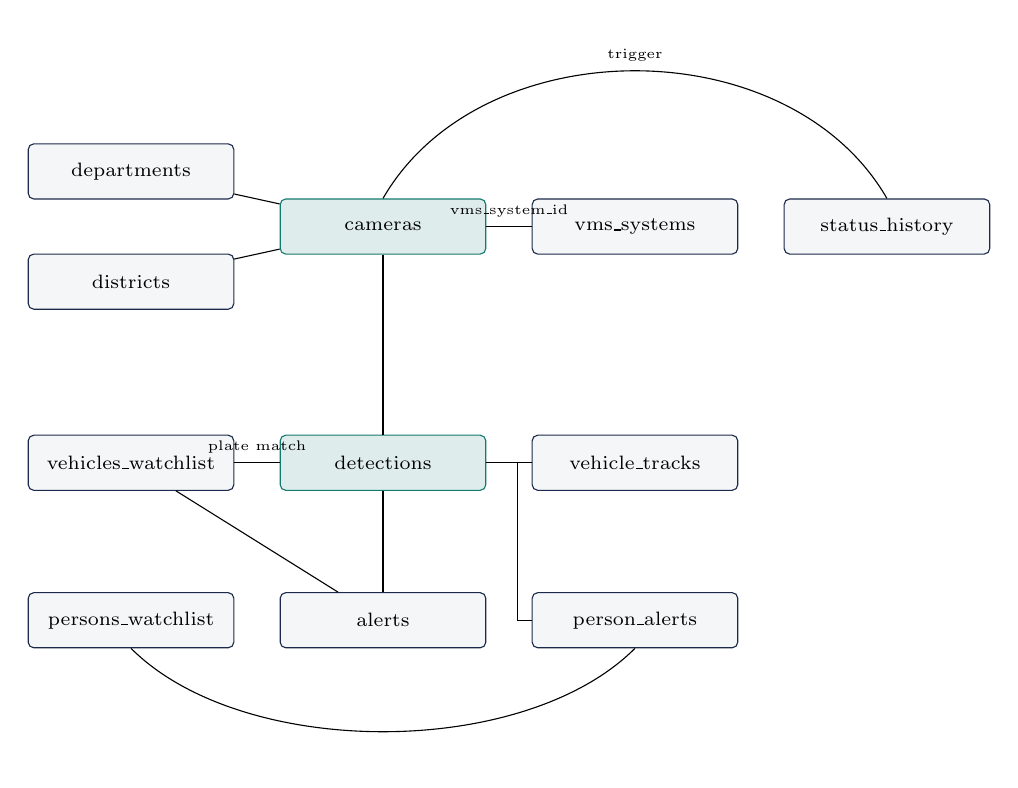
\begin{tikzpicture}[
  font=\scriptsize,
  ent/.style={draw, rounded corners=2pt, fill=lightbg, draw=navy, minimum height=0.7cm, text width=2.4cm, align=center, inner sep=3pt},
  core/.style={ent, fill=teal2!14, draw=teal2},
  >=Stealth
]

\node[ent] (dept) at (0,4.2) {departments};
\node[ent] (dist) at (0,2.8) {districts};
\node[core] (cam) at (3.2,3.5) {cameras};
\node[ent] (vms) at (6.4,3.5) {vms\_systems};

\node[ent] (vwl) at (0,0.5) {vehicles\_watchlist};
\node[core] (det) at (3.2,0.5) {detections};
\node[ent] (trk) at (6.4,0.5) {vehicle\_tracks};

\node[ent] (pwl) at (0,-1.5) {persons\_watchlist};
\node[ent] (alert) at (3.2,-1.5) {alerts};
\node[ent] (palert) at (6.4,-1.5) {person\_alerts};

\node[ent] (hist) at (9.6,3.5) {status\_history};

\draw (dept) -- (cam);
\draw (dist) -- (cam);
\draw (vms) -- (cam) node[midway, above, font=\tiny]{vms\_system\_id};
\draw (cam.north) to[out=60, in=120] node[midway, above, font=\tiny]{trigger} (hist.north);
\draw (cam) -- (det);
\draw (det) -- (trk);
\draw (vwl) -- (det) node[midway, above, font=\tiny]{plate match};
\draw (det) -- (alert);
\draw (vwl) -- (alert);
\draw (pwl.south) to[out=-45, in=-135, looseness=0.8] (palert.south);
\draw (det.east) -- ++(0.4,0) |- (palert.west);

\end{tikzpicture}

\caption{Simplified entity relationships across the shared schema. Full DDL is maintained separately in the codebase.}
\end{figure}

\end{document}
